\newpage

\subsection{QuizziPedia::Front-End::Views}
\subsubsection{Informazioni generali}
\label{QuizziPedia::Front-End}
\begin{figure}
	\centering
	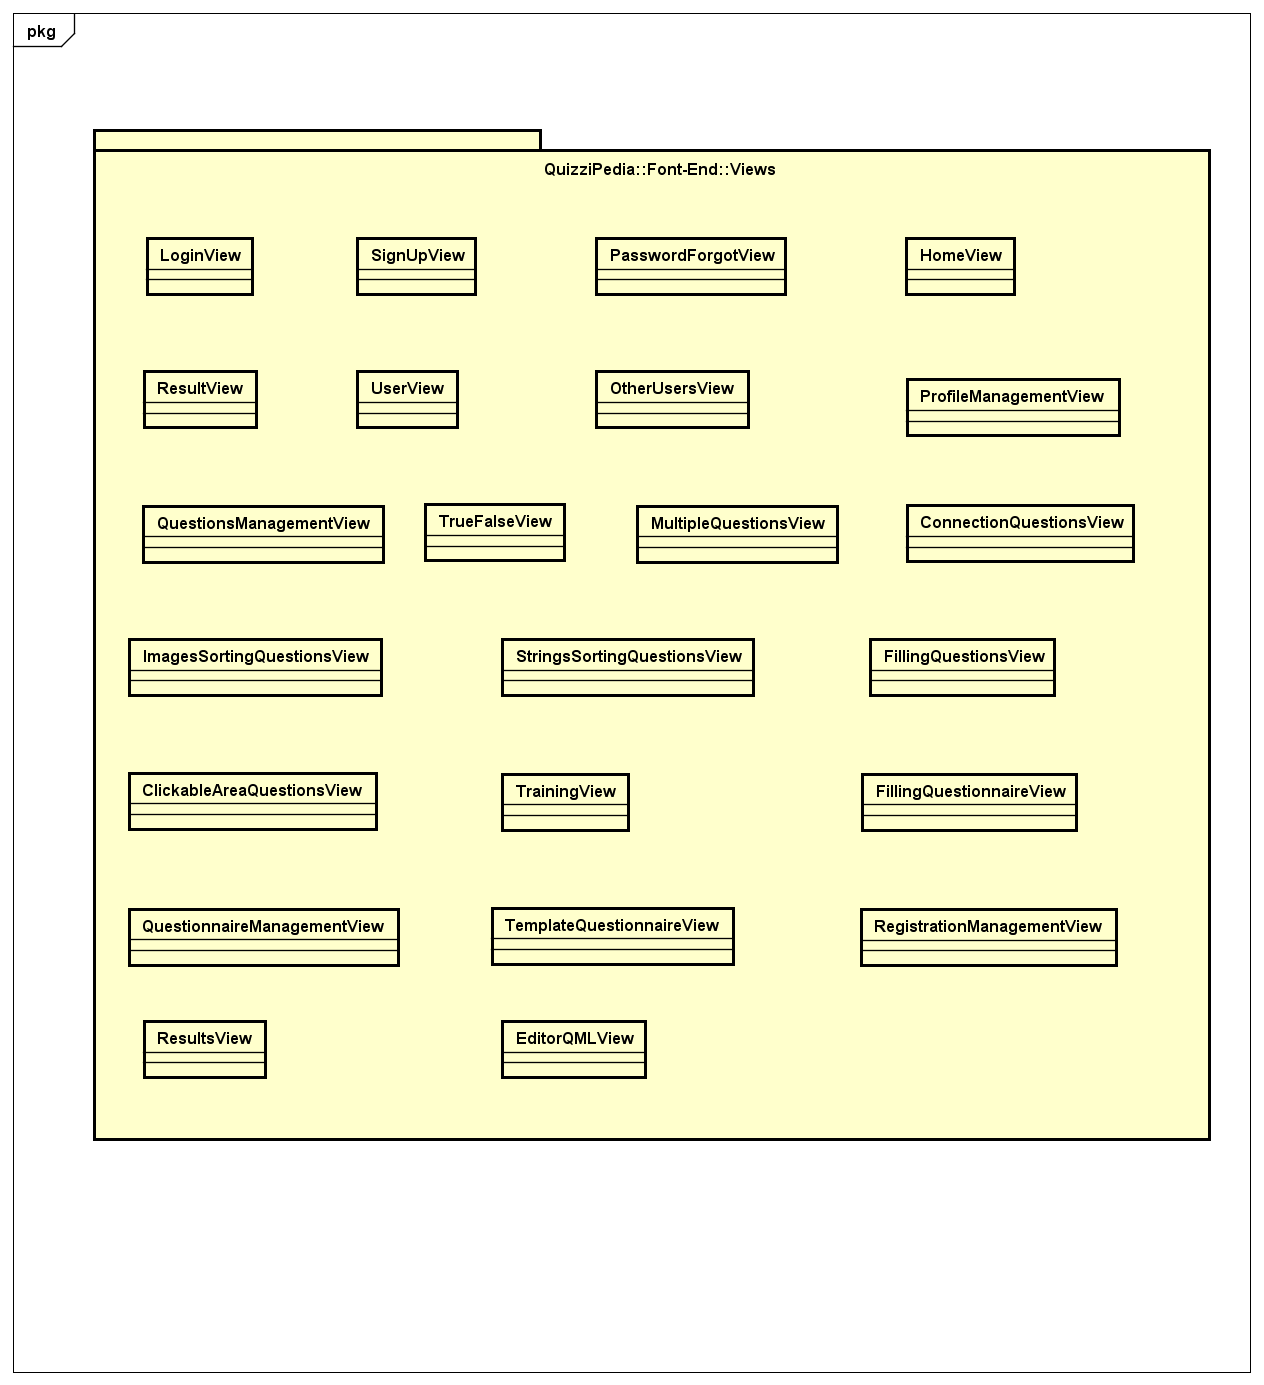
\includegraphics[scale=0.45]{UML/Package/QuizziPedia_Front-End_View.png}
	\caption{QuizziPedia::Front-End::Views}
\end{figure}
\begin{itemize}
	\item \textbf{Descrizione}
	Package contenente le views front-end dell'applicazione.
	\item \textbf{Padre}
	\texttt{Front-End}
	\item \textbf{Interazione con altri componenti}
	\item \texttt{Controllers} \\ Package contenente i controllers front-end dell'applicazione.
	\item \texttt{Directives} \\ Package contenente le directives front-end dell'applicazione.
	\item \texttt{Models} \\ Package contenente le classi che definiscono la business logic dell'applicazione.
	\item \texttt{Templates} \\ Package contenente i templates front-end dell'applicazione.
\end{itemize}
\subsubsection{Classi}

\paragraph{QuizziPedia::Front-End::Views::LoginView}
\begin{itemize}
	\item \textbf{Descrizione}: view contenente le form necessarie per effettuare il login. Contiene inoltre un link alla pagina di registrazione e uno alla pagina per il recupero della password;
	\item \textbf{Utilizzo}: premette all'utente di autenticarsi inserendo username e password;
	\item \textbf{Relazioni con altre classi}:
	\begin{itemize}
		\item \textit{IN} \texttt{LoginController} \\ 
	\end{itemize}
	\item \textbf{Attributi}
\end{itemize}

\paragraph{QuizziPedia::Front-End::Views::SignUpView}
\begin{itemize}
	\item \textbf{Descrizione}: view contenente le form dedicate alla registrazione utente. Contiene inoltre un link alla pagina di login;
	\item \textbf{Utilizzo}: permette all'utente di registrarsi al sistema inserendo i campi dati necessari;
	\item \textbf{Relazioni con altre classi}:
	\begin{itemize}
		\item \textit{IN} \texttt{SignUpController} \\
	\end{itemize}
	\item \textbf{Attributi}
\end{itemize}

\paragraph{QuizziPedia::Front-End::Views::PasswordForgotView}
\begin{itemize}
	\item \textbf{Descrizione}: view contenente le form necessarie per il recupero della password dimenticata;
	\item \textbf{Utilizzo}: permette all'utente di recuperare la password dimenticata inserendo i campi dati necessari, assieme alla nuova password inviatagli automaticamente dal sistema all'interno di una mail;
	\item \textbf{Relazioni con altre classi}:
	\begin{itemize}
		\item \textit{IN} \texttt{PasswordForgotController} \\
	\end{itemize}
	\item \textbf{Attributi}
\end{itemize}

\paragraph{QuizziPedia::Front-End::Views::HomeView}
\begin{itemize}
	\item \textbf{Descrizione}: view contenente la barra di ricerca per gli utenti e questionari e il bottone che porterà l'utente nella modalità allenamento;
	\item \textbf{Utilizzo}: viene utilizzata come view iniziale dell'applicazione;
	\item \textbf{Relazioni con altre classi}:
	\begin{itemize}
		\item \textit{IN} \texttt{HomeController} \\
		\item \textit{OUT} \texttt{SearchDirective} \\
	\end{itemize}
	\item \textbf{Attributi}
\end{itemize}
	
\paragraph{QuizziPedia::Front-End::Views::ResultView}
\begin{itemize}
	\item \textbf{Descrizione}: view contenente i risultati della ricerca effettuata, sia gli utenti che i questionari;
	\item \textbf{Utilizzo}: viene visualizzata dopo aver effettuato la ricerca di un utente o di un questionario nella barra di ricerca presente nella HomeView e permette di selezionare un risultato presente al suo interno; 
	\item \textbf{Relazioni con altre classi}:
	\begin{itemize}
		\item \textit{IN} \texttt{SearchController} \\
		\item \textit{OUT} \texttt{SubscribeResultDirective} \\
		\item \textit{OUT} \texttt{UserResultDirective} \\ 
	\end{itemize}
	\item \textbf{Attributi}
\end{itemize}

\paragraph{QuizziPedia::Front-End::Views::UserView}
\begin{itemize}
	\item \textbf{Descrizione}: view contenente i dati personali dell'utente, le sue statistiche relative ai questionari e agli allenamenti effettuati e i questionari a cui è iscritto;
	\item \textbf{Utilizzo}:  permette ad un utente di visualizzare i propri dati personali e le proprie statistiche e di controllare a quali questionari è iscritto. 
	\item \textbf{Relazioni con altre classi}:
	\begin{itemize}
		\item \textit{OUT} \texttt{StatisticsDirective}
		\item \textit{OUT} \texttt{UserDetailsDirective}
		\item \textit{OUT} \texttt{QuestionariDetailsDirective}
	\end{itemize}
	\item \textbf{Attributi}
\end{itemize}

\paragraph{QuizziPedia::Front-End::Views::OtherUserView}
\begin{itemize}
	\item \textbf{Descrizione}: view contenente i dati personali e le statistiche di un utente ricercato;
	\item \textbf{Utilizzo}: viene visualizzata dopo la ricerca di un utente e permette all'utente che ha effettuato la ricerca di visualizzare i dati personali e le statistiche di un utente ricercato;
	\item \textbf{Relazioni con altre classi}:
	\begin{itemize}
		\item \textit{OUT} \texttt{StatisticsDirective}
		\item \textit{OUT} \texttt{UserDetailsDirective}
	\end{itemize}
	\item \textbf{Attributi}
\end{itemize}

\paragraph{QuizziPedia::Front-End::Views::ProfileManagementView}
\begin{itemize}
	\item \textbf{Descrizione}: view contenente i dati personali che un utente può modificare dopo essersi registrato al sistema;
	\item \textbf{Utilizzo}: permette all'utente di modificare tutti i campi elencati e di rendere persistenti queste modifiche se sono accettate dal sistema;
	\item \textbf{Relazioni con altre classi}:
	\begin{itemize}
		\item \textit{IN} \texttt{ProfileManagementController} \\
	\end{itemize}
	\item \textbf{Attributi}
\end{itemize}

\paragraph{QuizziPedia::Front-End::Views::QuestionsManagementView}
\begin{itemize}
	\item \textbf{Descrizione}: view contenente l'elenco delle domande create; 
	\item \textbf{Utilizzo}: visualizza l'elenco delle domande create permettendo all'utente di crearne una nuova e di modificarne una presente nell'elenco;
	\item \textbf{Relazioni con altre classi}:
	\begin{itemize}
		\item \textit{IN} \texttt{QuestionsManagementController} \\
		\item \textit{OUT} \texttt{OneQuestionDirective} \\
		\item \textit{OUT} \texttt{NewQuestionButtonsDirective} \\ 
	\end{itemize}
	\item \textbf{Attributi}
\end{itemize}

\paragraph{QuizziPedia::Front-End::Views::TrueFalseQuestionsView}
\begin{itemize}
	\item \textbf{Descrizione}: view contenente i campi per creare una domanda vero/falso; 
	\item \textbf{Utilizzo}: permette all'utente di creare una domanda vero/falso compilando i campi proposti;
	\item \textbf{Relazioni con altre classi}:
	\begin{itemize}
		\item \textit{IN} \texttt{TrueFalseQuestionsController} \\
		\item \textit{OUT} \texttt{TopicKeywordsDirective} \\
		\item \textit{OUT} \texttt{ImageInTheQuestionDirective} \\
		\item \textit{OUT} \texttt{QuestionTextDirective} \\
		\item \textit{OUT} \texttt{AnswerChoiceDirective} \\   
	\end{itemize}
\item \textbf{Attributi}
\end{itemize}

\paragraph{QuizziPedia::Front-End::Views::MultipleQuestionsView}
\begin{itemize}
	\item \textbf{Descrizione}: view contenente i campi per creare una domanda a risposta multipla;
	\item \textbf{Utilizzo}: permette all'utente di creare una domanda a risposta multipla compilando i campi proposti;
	\item \textbf{Relazioni con altre classi}:
		\begin{itemize}
			\item \textit{IN} \texttt{MultiplyQuestionsController} \\
			\item \textit{OUT} \texttt{TopicKeywordsDirective} \\
			\item \textit{OUT} \texttt{ImageInTheQuestionDirective} \\
			\item \textit{OUT} \texttt{QuestionTextDirective} \\
			\item \textit{OUT} \texttt{AnswerChoiceDirective} \\   
		\end{itemize}
	\item \textbf{Attributi}
\end{itemize}

\paragraph{QuizziPedia::Front-End::Views::ConnectionQuestionsView}
\begin{itemize}
	\item \textbf{Descrizione}: view contenente i campi per creare una domanda a collegamento;
	\item \textbf{Utilizzo}: permette all'utente di creare una domanda a collegamento compilando i campi proposti;
	\item \textbf{Relazioni con altre classi}:
	\begin{itemize}
		\item \textit{IN} \texttt{ConnectionQuestionsController} \\
		\item \textit{IN} \texttt{InputToListController} \\
		\item \textit{OUT} \texttt{TopicKeywordsDirective} \\
		\item \textit{OUT} \texttt{QuestionTextDirective} \\ 
	\end{itemize}
	\item \textbf{Attributi}
\end{itemize}

\paragraph{QuizziPedia::Front-End::Views::ImagesSortingQuestionsView}
\begin{itemize}
	\item \textbf{Descrizione}: view contenente i campi per creare una domanda a ordinamento immagini;
	\item \textbf{Utilizzo}: permette all'utente di creare una domanda a ordinamento immagini compilando i campi proposti;
	\item \textbf{Relazioni con altre classi}:
	\begin{itemize}
		\item \textit{IN} \texttt{ImagesSortingQuestionsController} \\
		\item \textit{IN} \texttt{InputToListController} \\
		\item \textit{OUT} \texttt{ImageInTheQuestionDirective} \\
		\item \textit{OUT} \texttt{TopicKeywordsDirective} \\
		\item \textit{OUT} \texttt{QuestionTextDirective} \\ 
	\end{itemize}
	\item \textbf{Attributi}
\end{itemize}

\paragraph{QuizziPedia::Front-End::Views::StringsSortingQuestionsView}
\begin{itemize}
	\item \textbf{Descrizione}: view contenente i campi per creare una domanda a ordinamento stringhe;
	\item \textbf{Utilizzo}: permette all'utente di creare una domanda a ordinamento stringhe compilando i campi proposti;
	\item \textbf{Relazioni con altre classi}:
		\begin{itemize}
			\item \textit{IN} \texttt{StringsSortingQuestionsController} \\
			\item \textit{IN} \texttt{InputToListController} \\
			\item \textit{OUT} \texttt{TopicKeywordsDirective} \\
			\item \textit{OUT} \texttt{QuestionTextDirective} \\ 
		\end{itemize}
	\item \textbf{Attributi}
\end{itemize}

\paragraph{QuizziPedia::Front-End::Views::FillingQuestionsView}
\begin{itemize}
	\item \textbf{Descrizione}: view contenente i campi per creare una domanda a riempimento testo;
	\item \textbf{Utilizzo}:  permette all'utente di creare una domanda a riempimento testo compilando i campi proposti;
	\item \textbf{Relazioni con altre classi}:
	\begin{itemize}
		\item \textit{IN} \texttt{FillingQuestionsController} \\
		\item \textit{OUT} \texttt{TopicKeywordsDirective} \\
		\item \textit{OUT} \texttt{QuestionTextDirective} \\ 
	\end{itemize}
	\item \textbf{Attributi}
\end{itemize}

\paragraph{QuizziPedia::Front-End::Views::ClickableAreaQuestionsView}
\begin{itemize}
	\item \textbf{Descrizione}: view contenente i campi per creare una domanda ad area cliccabile;
	\item \textbf{Utilizzo}:  permette all'utente di creare una domanda ad area cliccabile compilando i campi proposti;
	\item \textbf{Relazioni con altre classi}:
	\begin{itemize}
		\item \textit{IN} \texttt{ClickableAreaQuestionsController} \\
		\item \textit{OUT} \texttt{ImageInTheQuestionDirective} \\
		\item \textit{OUT} \texttt{TopicKeywordsDirective} \\
		\item \textit{OUT} \texttt{QuestionTextDirective} \\ 
	\end{itemize}
	\item \textbf{Attributi}
\end{itemize}

\paragraph{QuizziPedia::Front-End::Views::EditorQMLView}
\begin{itemize}
	\item \textbf{Descrizione}: view contenente l'editor QML per la creazione di domande personalizzate;
	\item \textbf{Utilizzo}: permette ad un utente di creare domande personalizzate attraverso la scrittura del codice QML direttamente nell'editor di testo presente nella view;
	\item \textbf{Relazioni con altre classi}:
	\begin{itemize}
		\item \textit{IN} \texttt{EditorQMLController} \\
	\end{itemize}
	\item \textbf{Attributi}
\end{itemize}

\paragraph{QuizziPedia::Front-End::Views::TrainingView}
\begin{itemize}
	\item \textbf{Descrizione}
	\item \textbf{Utilizzo}
	\item \textbf{Relazioni con altre classi}
	\item \textbf{Attributi}
\end{itemize}

\paragraph{QuizziPedia::Front-End::Views::FillingQuestionnaireView}
\begin{itemize}
	\item \textbf{Descrizione}
	\item \textbf{Utilizzo}
	\item \textbf{Relazioni con altre classi}
	\item \textbf{Attributi}
\end{itemize}

\paragraph{QuizziPedia::Front-End::Views::QuestionnaireManagementView}
\begin{itemize}
	\item \textbf{Descrizione}
	\item \textbf{Utilizzo}
	\item \textbf{Relazioni con altre classi}
	\item \textbf{Attributi}
\end{itemize}

\paragraph{QuizziPedia::Front-End::Views::TemplateQuestionnaireView}
\begin{itemize}
	\item \textbf{Descrizione}
	\item \textbf{Utilizzo}
	\item \textbf{Relazioni con altre classi}
	\item \textbf{Attributi}
\end{itemize}

\paragraph{QuizziPedia::Front-End::Views::RegistrationManagementView}
\begin{itemize}
	\item \textbf{Descrizione}
	\item \textbf{Utilizzo}
	\item \textbf{Relazioni con altre classi}
	\item \textbf{Attributi}
\end{itemize}

\paragraph{QuizziPedia::Front-End::Views::ResultsView}
\begin{itemize}
	\item \textbf{Descrizione}
	\item \textbf{Utilizzo}
	\item \textbf{Relazioni con altre classi}
	\item \textbf{Attributi}
\end{itemize}